\documentclass[lang=cn,11pt,a4paper]{elegantpaper}


\usepackage{graphicx}
\usepackage{fancyhdr}

%导入数据库的参考文献模板
\bibliographystyle{plain}

\newcommand\course{智能计算系统}
\pagestyle{fancyplain}

\title{仿真报告}
\author{王磊 2021E8013282048 \\ }
\institute{\href{http://www.ict.ac.cn/}{中国科学院计算技术研究所}}

\headheight 30pt
\lhead{
\includegraphics[height=1cm]{logo.jpg}}
\rhead{\course\\ \today}
\lfoot{}

\date{\zhtoday}

\usepackage{appendix}
\renewcommand{\appendixtocname}{附录}
\renewcommand{\appendixpagename}{附录}
\newcommand{\upcite}[1]{\textsuperscript{\textsuperscript{\cite{#1}}}}

\begin{document}
\maketitle



\section{serial pe}

串行PE的仿真波形如图~\ref{fig:serial-result}所示,可以观察到PE运算阵列的输出与期望输出结果一致,能够正常工作。

\begin{figure}[!htbp]
  \centering
  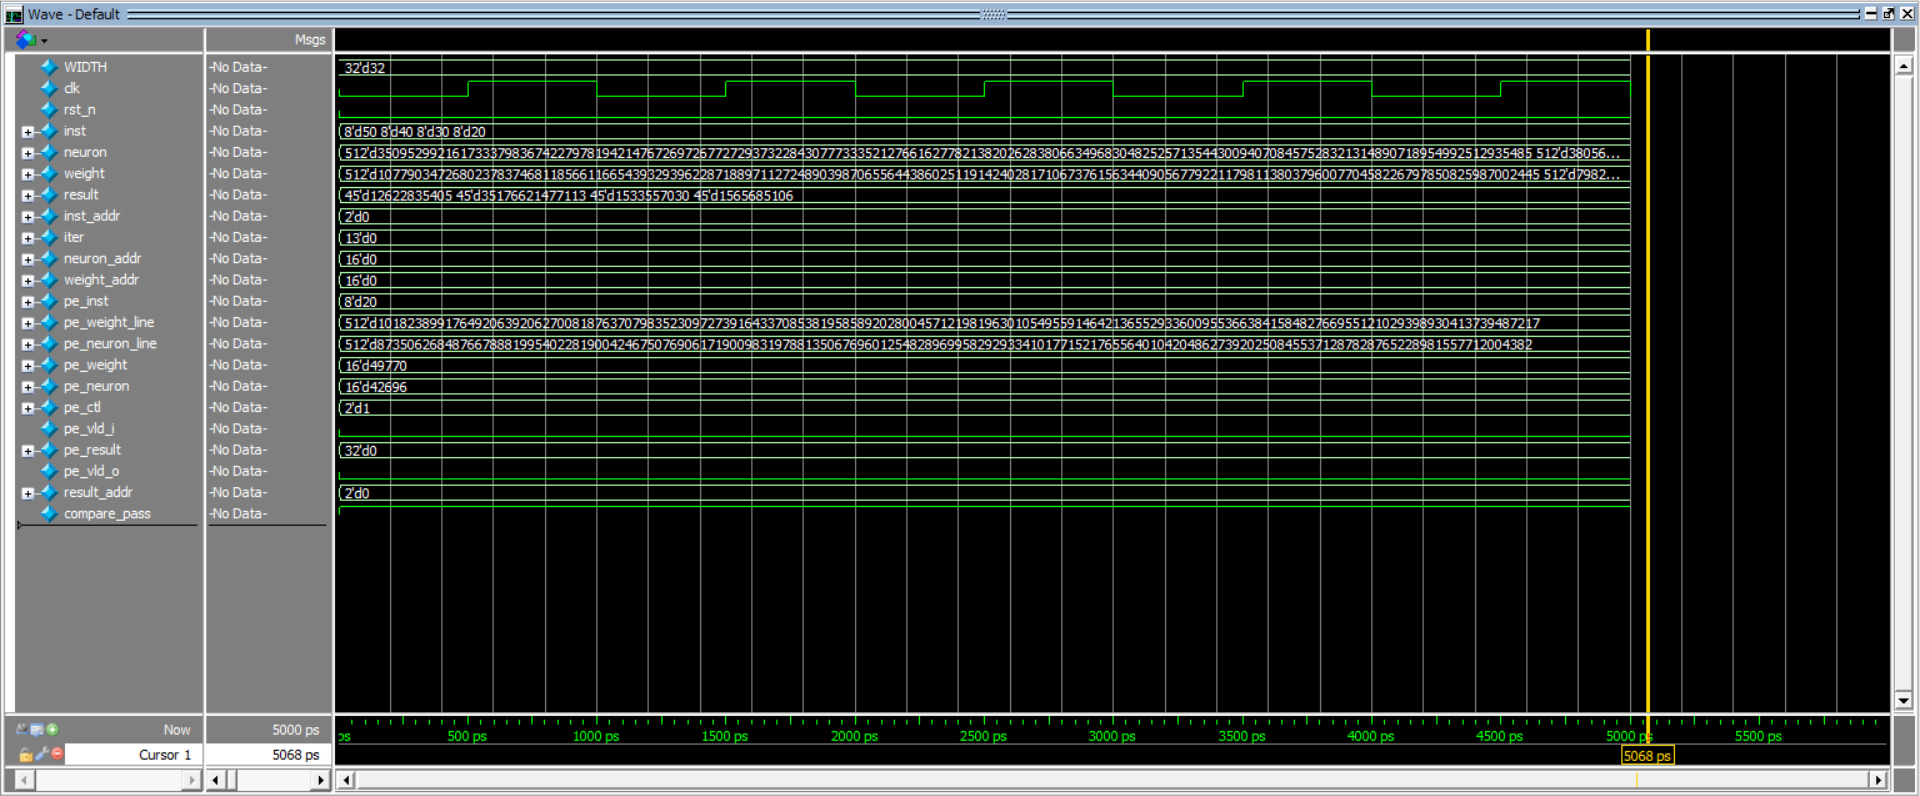
\includegraphics[width=1.0\textwidth]{image/serial.png}
  \caption{Seiral PE simlation wave}
  \label{fig:serial-result}
\end{figure}


\section{parallel pe}

并行PE的仿真波形如图~\ref{fig:parallel-result}所示,可以观察到PE运算阵列的输出与期望输出结果一致,能够正常工作。

\begin{figure}[!htbp]
  \centering
  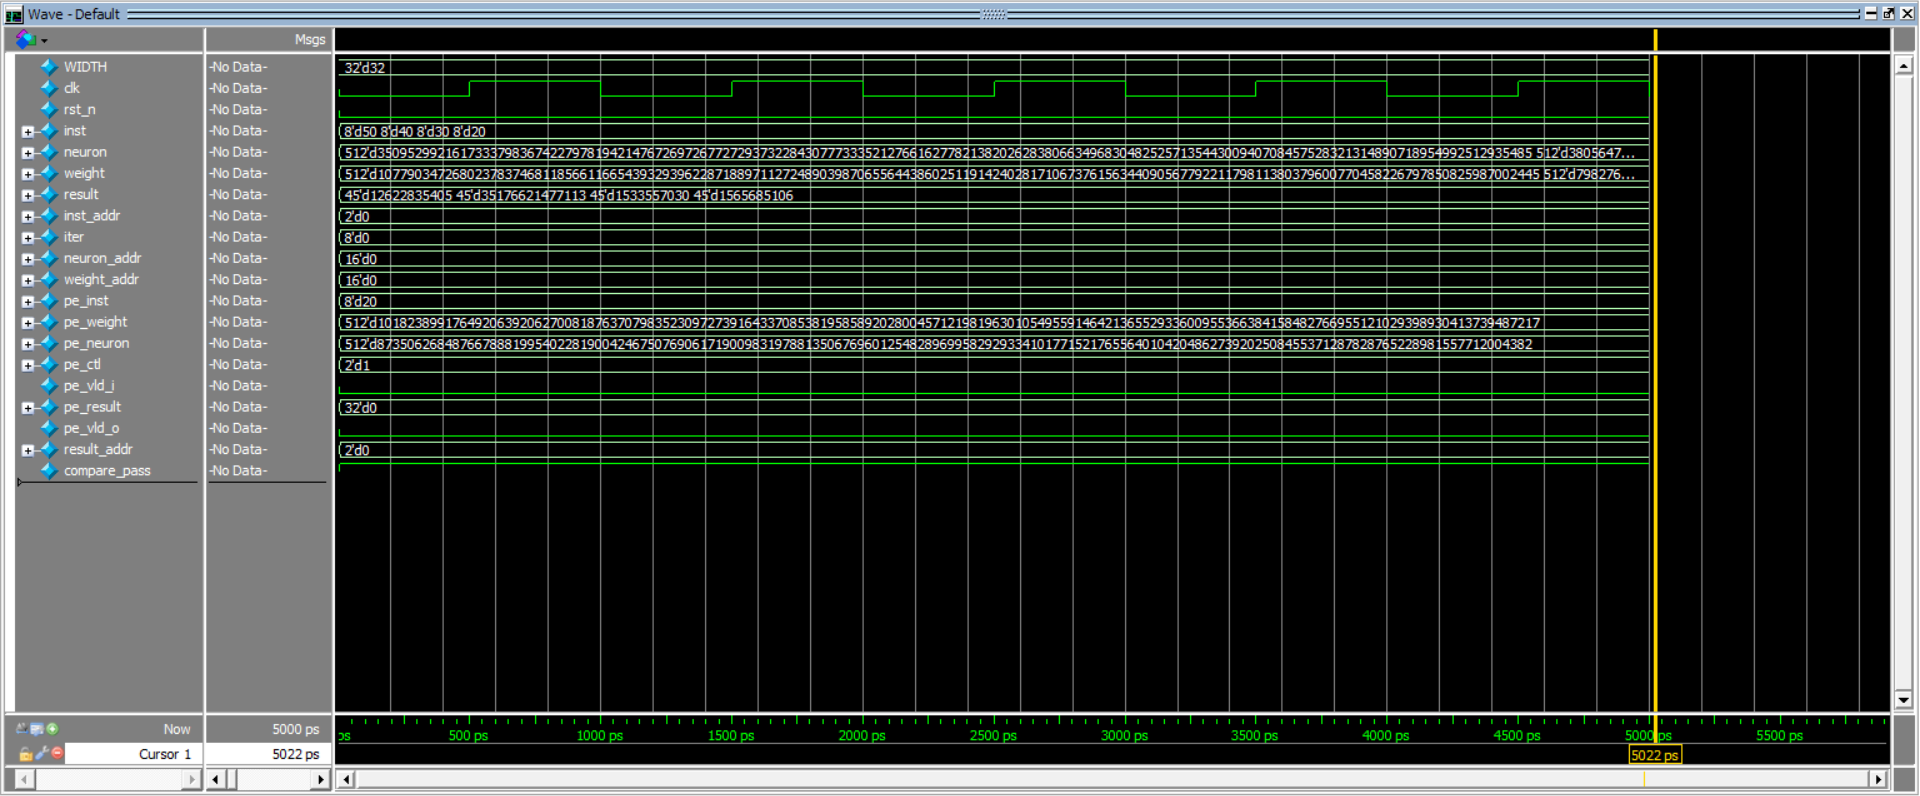
\includegraphics[width=1.0\textwidth]{image/parallel.png}
  \caption{Parallel PE simlation wave}
  \label{fig:parallel-result}
\end{figure}

\pagebreak
\section{matrix pe}

二维PE阵列的仿真波形如图~\ref{fig:matrix-result}所示,可以观察到PE运算阵列的输出与期望输出结果一致,能够正常工作。

\begin{figure}[!htbp]
  \centering
  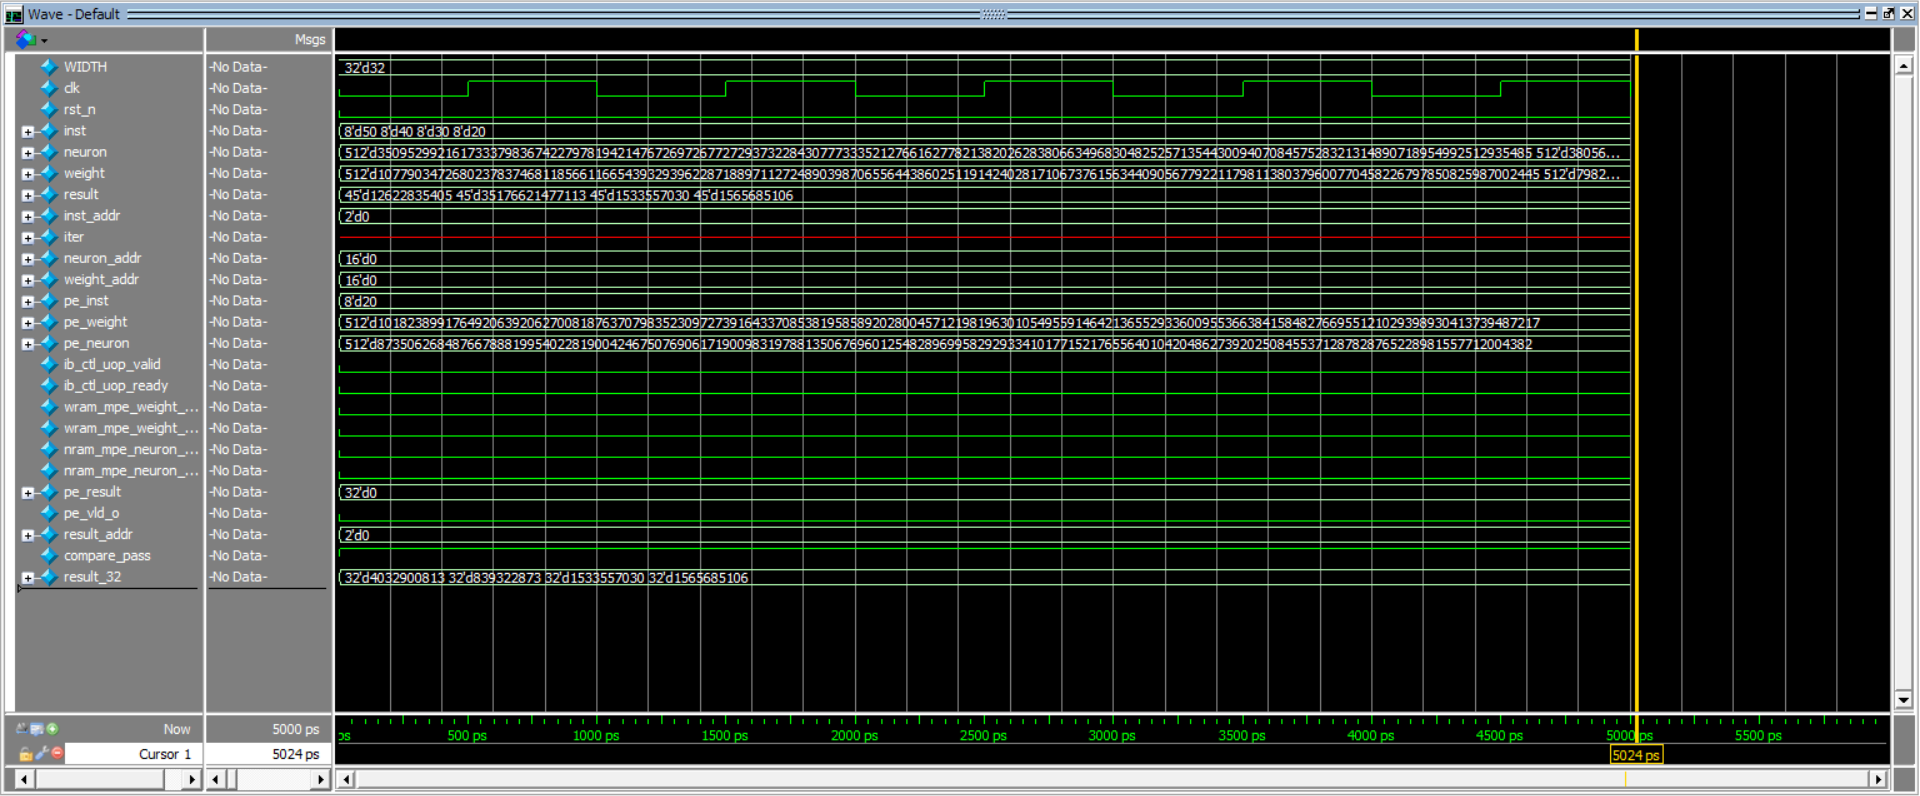
\includegraphics[width=1.0\textwidth]{image/matrix.png}
  \caption{Matrix PE simlation wave}
  \label{fig:matrix-result}
\end{figure}

% \pagebreak

% \bibliography{ref.bib}

\end{document}
